\chapter{Introduction}
\label{intro}

The future is arriving faster than we think. The technological progress is accelerating. Human knowledge is growing faster than ever before. If citing slightly lurid sources, according to Fuller's knowledge doubling curve \cite{knowledge-doubling-curve}, it took about 1500 years starting at the year 1 for the society amount of knowledge to double itself, then the doubling needed just about 100 years around the year 1900, and only 10 years around the year 1960; according to \cite{growth-forecast}, the knowledge doubled every 1.5 years around the year 2011. Besides many other aspects of such an information growth, it opens gates for technologies previously only dreamed up. Technologies like the artificial intelligence (\zk{AI}).

Artificial neural networks (\zk{ANN}s) became a term that is shaking the entire field of computer science. In the field of computer vision, it is especially their special type called convolutional neural networks (\zk{CNN}s) that is outperforming classical approaches to object detection and segmentation \cite{cnn-off-the=shelf}. Therefore, it should not be a surprise that \zk{ANN}s are widely used also in the field of remote sensing already since 2014 \cite{review-dl-rs-2017}, and their use outside and inside the field is just growing, as can be seen in figures \ref{fig-dl} and \ref{fig-rs-dl}.

\begin{figure}[h]
   \centering
	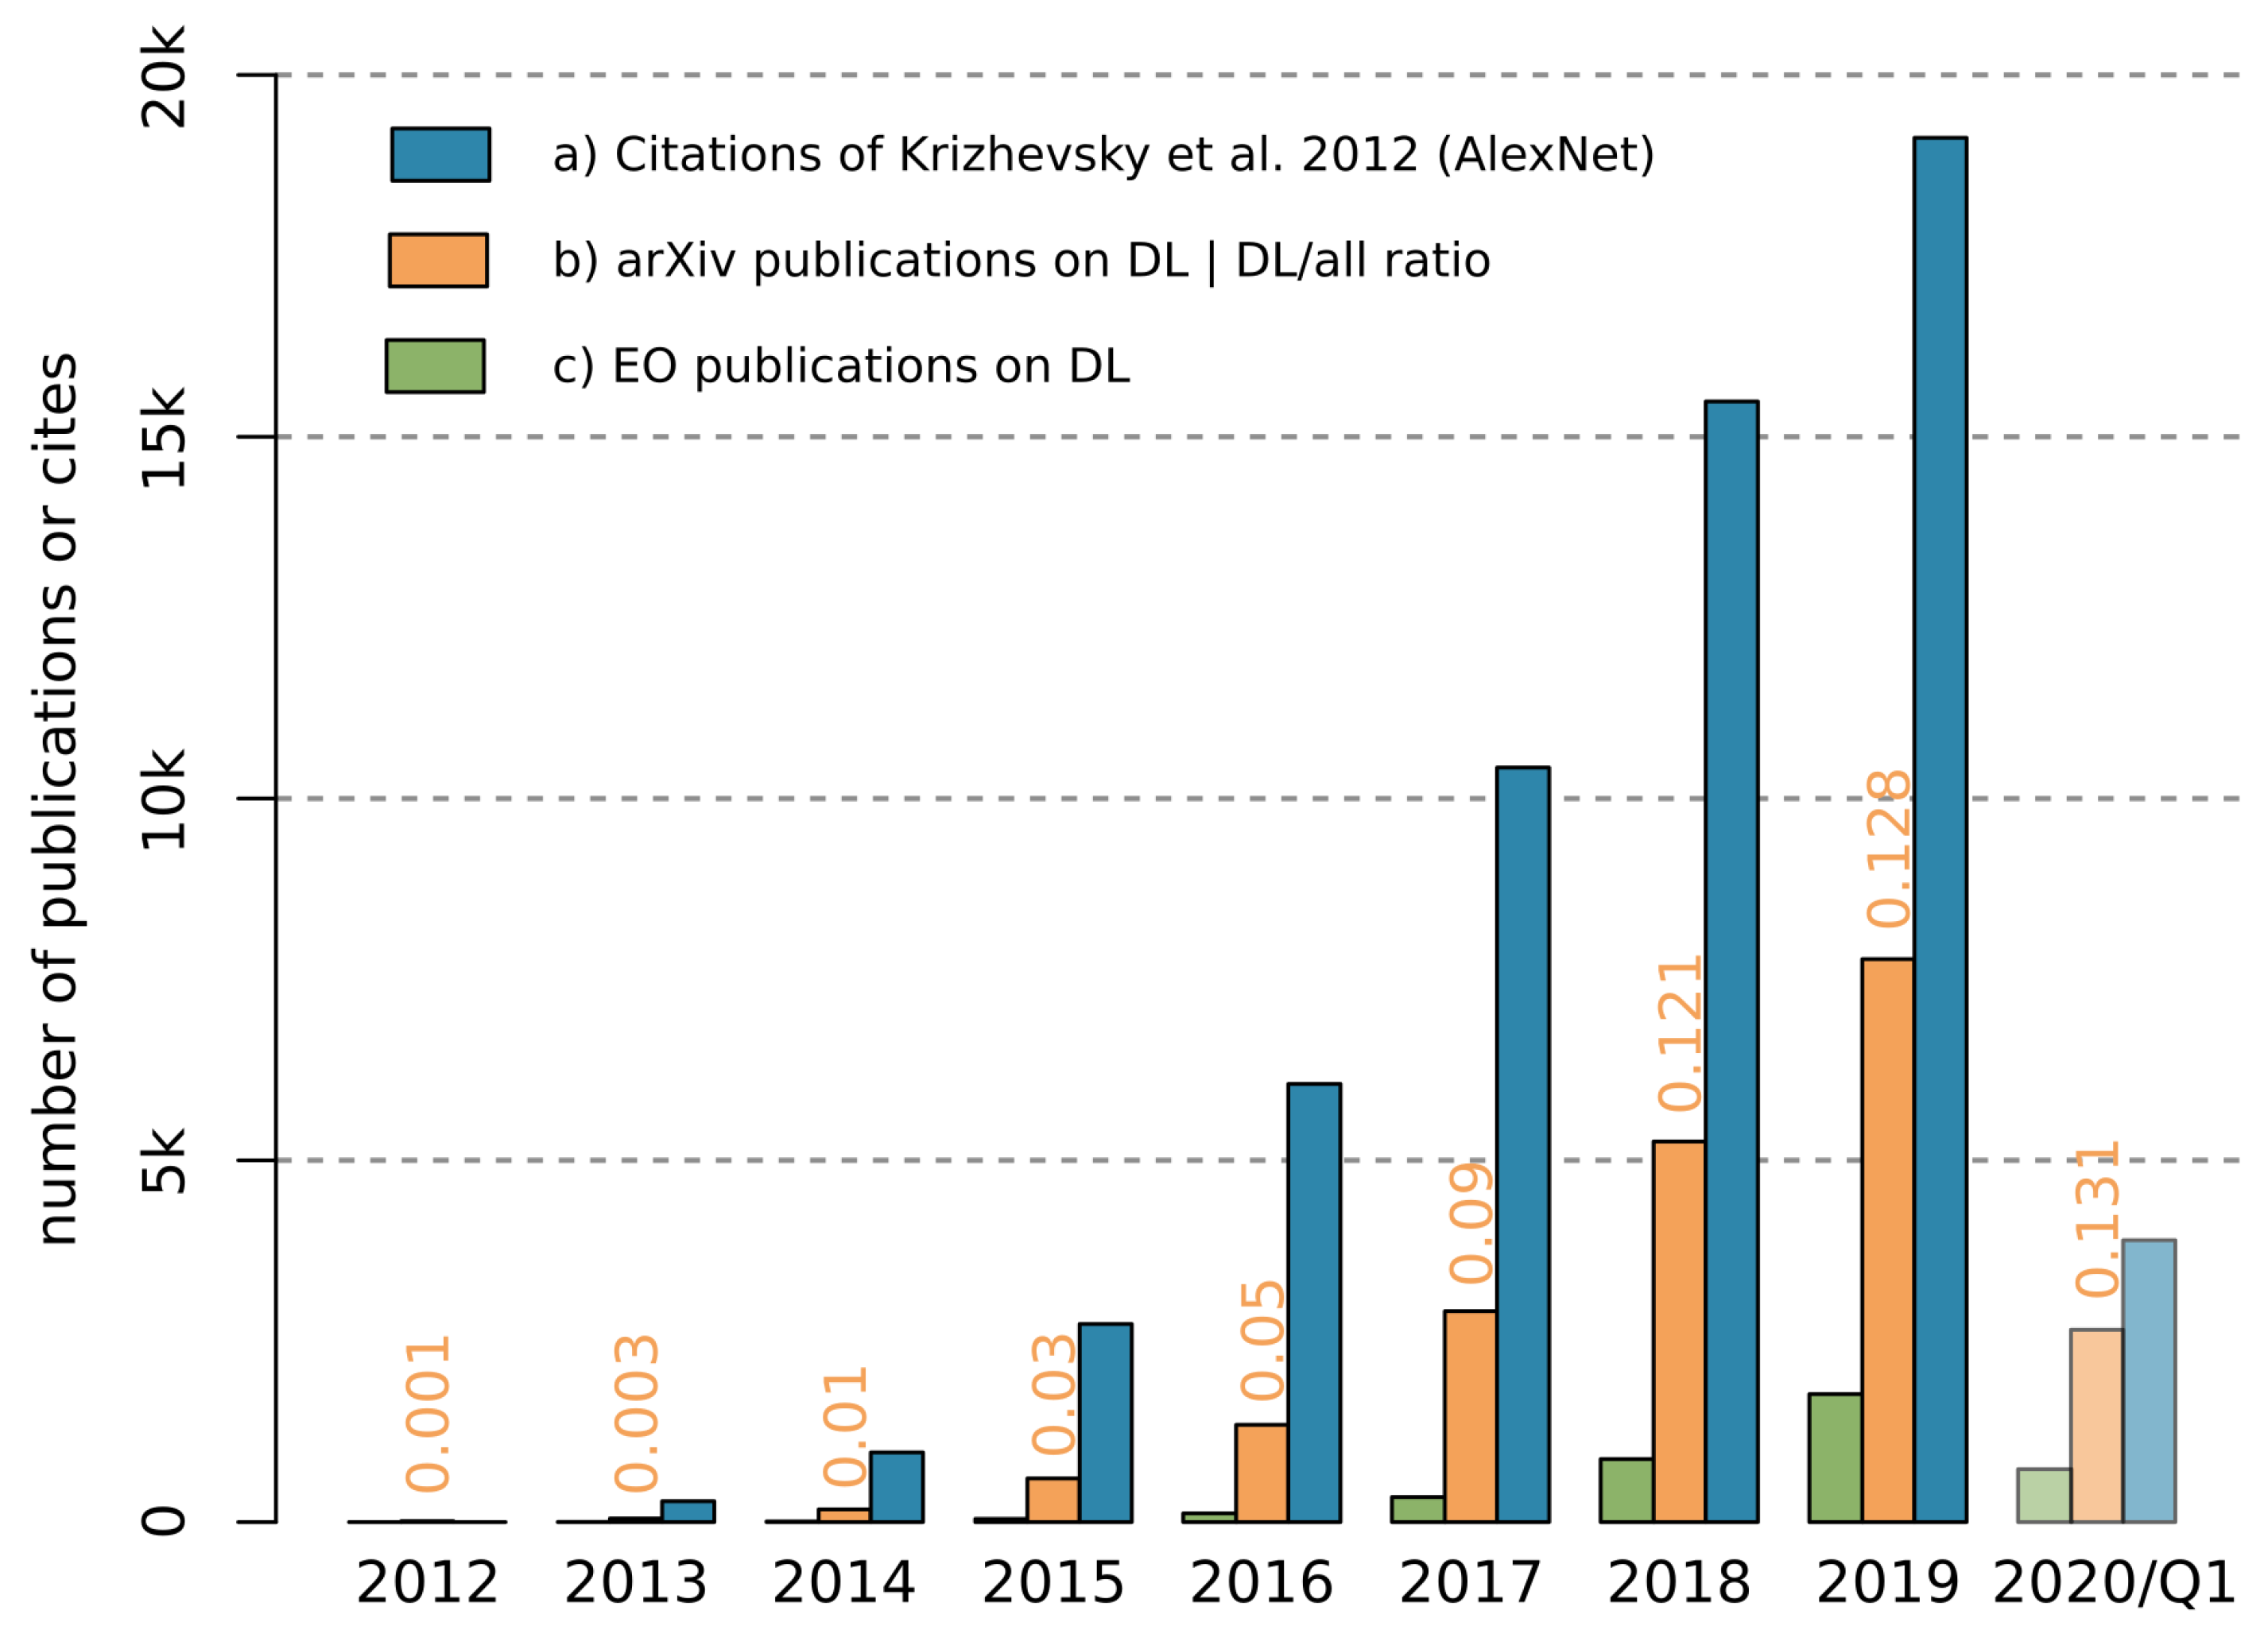
\includegraphics[width=0.6\linewidth]{./pictures/dl-papers.png}
	\caption[Papers on the use of DL]{Statistics for papers dealing with the use of deep learning in remote sensing: Citations listed in Google scholar for famous \zk{CNN} architecture \cite{cnn-classification}; arXiv listed publications in the categories \textit{cs} and \textit{stat} including the terms \textit{deep learning}, \textit{convolutional neural networks}, \textit{convolutional networks} or \textit{fully convolutional} and their share of all publications listed in the two categories; publications in selected Earth observation journals, searched for with the same terms as in arXiv, source: \cite{review-dl-eo}}
      \label{fig-dl}
\end{figure}

\begin{figure}[h]
   \centering
	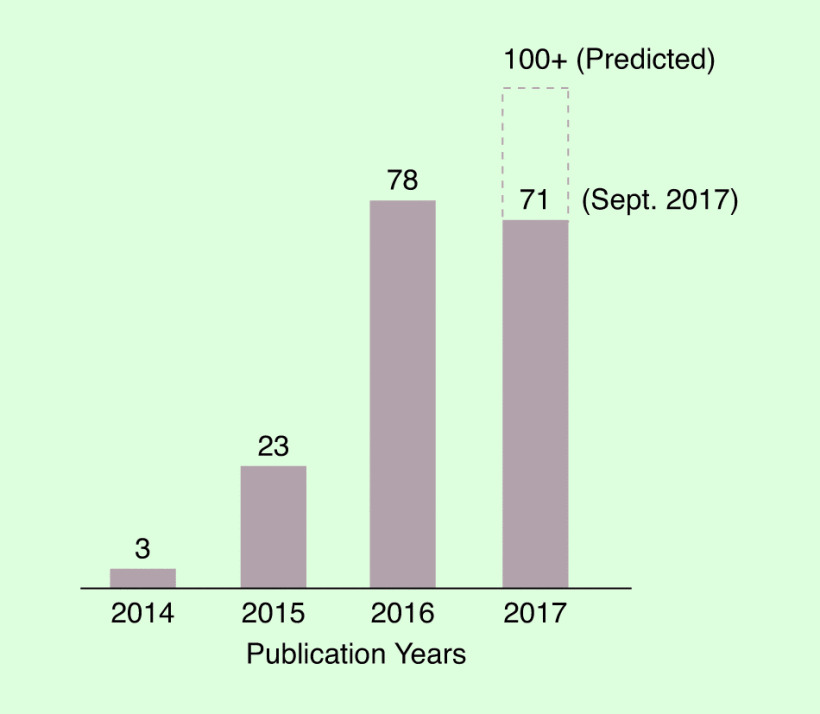
\includegraphics[width=0.6\linewidth]{./pictures/dl-rs-papers.jpg}
	\caption[Papers on the use of DL in remote sensing]{Number of papers dealing with the use of deep learning in remote sensing per year, source: \cite{review-dl-rs-2017}}
      \label{fig-rs-dl}
\end{figure}

However, this quick development of \zk{ANN}s and \zk{CNN}s makes it harder and harder for other fields as remote sensing to keep up with the progress tempo. It results in the situation where when it comes to an \zk{ANN} architecture choose, researchers without the necessary background simply choose the newest one or the one with the best reported results, although these results could be obtained on completely different data in a completely different environment and the performance could therefore very much differ from the expected one. The goal of this thesis is to try to make complex, systematic research and review of the performance of chosen \zk{CNN} architectures on various selected use cases from the field of remote sensing, and hopefully serve as a valuable guidebook when it comes to \zk{CNN} applications in the field or comparison metrics when a new architecture is proposed.

Chapter \ref{motivation} will present research on the use of comparisons when it comes to papers dealing with \zk{CNN} models in the field of remote sensing and systematically investigate their senses of comparing the original input with the already existing work from different points of view to give them sufficient scientific context. The same systematical investigation will be done also for reviews of the use of \zk{CNN}s in the field.

% TODO: Delete info about the professional debate
Chapter \ref{use-cases} will present use cases selected as test tasks to evaluate chosen architectures. For purposes of the professional debate, only one use case is presented.

These chapters will be later followed by a chapter on selected architectures and methods and a chapter presenting the results of the experiments. For purposes of the professional debate, these are not present.